% !TEX program = pdflatex
\documentclass[11pt,a4paper]{article}

% ============ Layout ============
\usepackage[top=2.5cm,bottom=2.5cm,left=2.5cm,right=2.5cm]{geometry}
\usepackage{setspace}
\onehalfspacing

% ============ Figures & Tables ============
\usepackage{graphicx}
\usepackage{booktabs}
\usepackage{multirow}
\usepackage{array}

% ============ Math ============
\usepackage{amsmath,amssymb,bm}
\DeclareMathOperator*{\argmax}{arg\,max}
\DeclareMathOperator*{\argmin}{arg\,min}

% ============ Citations ============
\usepackage[numbers,sort&compress]{natbib}
\usepackage{hyperref}
\hypersetup{colorlinks=true,linkcolor=blue,citecolor=blue,urlcolor=blue}

% ============ Misc ============
\usepackage{algorithm}
\usepackage{algorithmic}
\usepackage{color}

% ============ Title ============
\title{\bfseries HardBPR: Semantic-Aware Bayesian Personalized Ranking\\for Collaborative Filtering}
\author{Zhaoyang Zhang\thanks{School of Statistics, Southeast University, Nanjing 211189, China. Email: \texttt{yourname@seu.edu.cn}}}
\date{\today}

\begin{document}
\maketitle

\begin{abstract}
While large language model (LLM) embeddings have been widely adopted to enhance collaborative filtering recommenders, existing work focuses on injecting LLM semantics at the \emph{feature level}, leaving the training signal itself as an independent yet complementary bottleneck. We identify that standard Bayesian Personalized Ranking (BPR) loss treats all positive-negative sample pairs equally, causing the majority of training iterations to be spent on distinguishing semantically unrelated ``easy'' negatives (e.g., distinguishing a sci-fi novel from a cookbook). Unlike prior BPR enhancement methods that rely on model-internal scores or propensity estimation, we propose \emph{HardBPR}, which leverages frozen LLM item embeddings to compute pairwise semantic similarity for loss reweighting---without adding parameters, without modifying model architecture, and without any LLM inference overhead. Experiments on three public datasets (Amazon-Book, Steam, Yelp) demonstrate that HardBPR improves Recall@20 by 13.0\% on MF and 44.7\%--101.1\% on LightGCN over standard BPR training, while having negligible effect on models already saturating BPR optimization (e.g., NGCF). We further provide an Information Bottleneck analysis explaining why semantic signals are beneficial at the loss level yet harmful at the data level, establishing a design principle for future semantic enhancement methods.
\end{abstract}

% ============================================================
\section{Introduction}
% ============================================================

Collaborative filtering (CF) is a cornerstone technology for recommender systems. Models such as matrix factorization~\cite{Koren2009}, neural collaborative filtering~\cite{He2017NCF}, and graph-based collaborative filtering~\cite{He2020LightGCN} mine co-occurrence patterns from user-item interaction matrices to produce personalized recommendations. However, pure CF suffers from a fundamental semantic deficiency: items are merely ID indices, and the model cannot understand that ``\emph{The Three-Body Problem} is a sci-fi novel'' or that ``this user prefers hard science fiction.''

The recent emergence of large language models (LLMs) offers a path toward addressing this problem. RLMRec~\cite{Ren2024RLMRec} pioneered the use of LLM-generated user/item textual profiles encoded as semantic embeddings, injected into graph CF models via alignment losses. Subsequently, LLMInit~\cite{Zhang2025LLMInit}, RecMind~\cite{Xue2026RecMind}, DALR~\cite{Peng2024DALR}, and others have improved the fusion mechanisms from various angles.

However, these works share a common characteristic: while they carefully design how LLM semantic embeddings are injected into model architectures, they all inherit the \emph{same training paradigm}---standard BPR loss with uniform random negative sampling. This training paradigm has a bottleneck independent of feature design: the vast majority of randomly sampled negatives are semantically irrelevant to the positive sample. Distinguishing them contributes near-zero informative gradients, while the genuinely challenging negative samples (e.g., distinguishing \emph{Ball Lightning} from \emph{The Three-Body Problem}) are rarely encountered during training.

Our contributions are as follows:
\begin{enumerate}
    \item We propose \emph{HardBPR}, a training-time enhancement that modifies only the loss function with zero additional parameters. Frozen LLM semantic embeddings are used to compute the pairwise semantic similarity between positive and negative samples, and harder samples receive proportionally higher loss weights.
    \item We design two semantic-aware mechanisms: \emph{Weighted HardBPR} (amplifying loss weights for hard samples) and \emph{Margin HardBPR} (imposing stricter ranking margins), and experimentally verify that the weighted variant is superior.
    \item Through ablation studies on auxiliary enhancements---hot-to-cold collaborative distillation and semantic hard negative sampling---we discover that the former yields marginal gains while the latter is actually harmful, establishing that \emph{the optimal injection point for semantic signals is the loss level, not the data level}.
    \item We validate HardBPR across three datasets and three backbone architectures, demonstrating consistent improvements and providing an Information Bottleneck analysis that explains \emph{why} loss-level semantic injection works while data-level injection does not.
\end{enumerate}

% ============================================================
\section{Related Work}
% ============================================================

\subsection{Collaborative Filtering and LightGCN}

Early CF was dominated by matrix factorization (MF)~\cite{Koren2009}, which predicts ratings as the inner product of latent user and item vectors. BPR~\cite{Rendle2009} shifted the optimization objective from rating prediction to pairwise ranking under implicit feedback, defining the standard training paradigm for modern CF. NCF~\cite{He2017NCF} introduced neural networks to learn more complex user-item interaction functions. LightGCN~\cite{He2020LightGCN} further simplified the architecture by removing feature transformations and nonlinear activations from GCNs, retaining only normalized neighbor aggregation, demonstrating that ``less is more'' in recommendation scenarios lacking node features.

\subsection{LLM-Enhanced Recommendation}

The intersection of LLMs and recommender systems is a rapidly growing area. RLMRec~\cite{Ren2024RLMRec} is a foundational work: it uses ChatGPT to generate user/item textual profiles, encodes them into 1536-dimensional semantic vectors via text-embedding-ada-002, and aligns the collaborative and semantic spaces through contrastive (InfoNCE) or generative (masked reconstruction) losses. Its precomputed embeddings are widely adopted by subsequent works (including ours).

LLMInit~\cite{Zhang2025LLMInit} proposes the simplest injection scheme: initializing CF model ID embeddings with LLM text embeddings and training without further LLM signals. This adds no parameters or inference cost, though the initialization advantage decays during training.

RecMind~\cite{Xue2026RecMind} introduces a gating mechanism atop LightGCN that adaptively selects between semantic and collaborative signals for different items. DALR~\cite{Peng2024DALR} proposes denoising contrastive alignment that simultaneously bridges the semantic space gap and suppresses interaction noise. RecGOAT~\cite{Li2026RecGOAT} applies optimal transport theory to semantic alignment.

TAGCF~\cite{Meng2026TAGCF} represents an alternative paradigm: rather than using LLM embeddings, it uses LLM reasoning to generate attribute labels that restructure the user-item graph into a user-attribute-item tripartite topology.

\subsection{Improving BPR Training}

Beyond architectural work, several efforts directly improve BPR training. IPS-BPR~\cite{Raja2025IPS} reweights BPR with propensity scores to correct exposure bias. Hard-BPR~\cite{Shi2024HardBPR} redesigns the sigmoid gradient curve into a bell shape to suppress gradients from potential false negatives. ReFINe~\cite{Jeong2025ReFINe} uses LLMs to classify negative feedback as true/false and applies category-specific weights.

Our work differs fundamentally from these approaches: (1) we use \emph{continuous} cosine similarity from LLM embeddings for BPR reweighting, not binary classification or propensity estimation; (2) we do not alter the BPR gradient functional form, but rather apply semantically-guided sample weights on top of standard BPR; (3) we provide an Information Bottleneck analysis explaining the loss-level-vs-data-level disparity---a perspective unexplored in prior work.

% ============================================================
\section{Method}
% ============================================================

\subsection{Preliminaries: LightGCN}

We adopt LightGCN as the base architecture. LightGCN is a pure graph-based CF model whose node embeddings are randomly initialized and refined through $K$ layers of graph propagation:
\begin{equation}
    \mathbf{E}^{(k+1)} = \tilde{\mathbf{A}} \, \mathbf{E}^{(k)}, \quad k = 0,1,\dots,K-1
\end{equation}
where $\tilde{\mathbf{A}} = \mathbf{D}^{-1/2}\mathbf{A}\mathbf{D}^{-1/2}$ is the symmetric normalized adjacency matrix, and $\mathbf{E}^{(0)}$ is initialized from $\mathcal{N}(0, 0.1^2)$. The final representation is the layer-wise average:
\begin{equation}
    \mathbf{E} = \frac{1}{K+1} \sum_{k=0}^{K} \mathbf{E}^{(k)}
\end{equation}
The prediction score is the inner product: $\hat{y}_{ui} = \mathbf{e}_u^{\top} \mathbf{e}_i$.

\textbf{Crucially}, \textbf{no LLM features are introduced} anywhere in the forward pass---the model architecture is identical to standard LightGCN. Frozen LLM semantic embeddings serve solely as a ``semantic referee'' in the loss function described below.

\subsection{Standard BPR and Its Bottleneck}

The standard BPR loss is:
\begin{equation}
    \mathcal{L}_{\text{BPR}} = -\frac{1}{|\mathcal{D}|} \sum_{(u,i,j) \in \mathcal{D}} \ln \sigma(\hat{y}_{ui} - \hat{y}_{uj})
\end{equation}
where $\mathcal{D} = \{(u,i,j) \mid i \in \mathcal{I}_u^+, j \in \mathcal{I} \setminus \mathcal{I}_u^+\}$, and negative samples $j$ are drawn uniformly at random.

The BPR gradient is:
\begin{equation}
    \frac{\partial \mathcal{L}}{\partial \Theta} \propto (1 - \sigma(\Delta\hat{y})) \cdot \frac{\partial \Delta\hat{y}}{\partial \Theta}
\end{equation}
where $\Delta\hat{y} = \hat{y}_{ui} - \hat{y}_{uj}$. When the negative sample $j$ is semantically unrelated to the positive $i$ (e.g., a cookbook vs.\ a sci-fi novel), $\Delta\hat{y}$ is large, $\sigma(\Delta\hat{y}) \approx 1$, and the gradient approaches zero---these training samples contribute almost no useful learning signal.

Fig.~\ref{fig:grad} visualizes the gradient distribution: under standard BPR, the majority of samples concentrate near zero gradient (``easy'' samples), while only a small fraction produce informative large gradients.

\begin{figure}[ht]
    \centering
    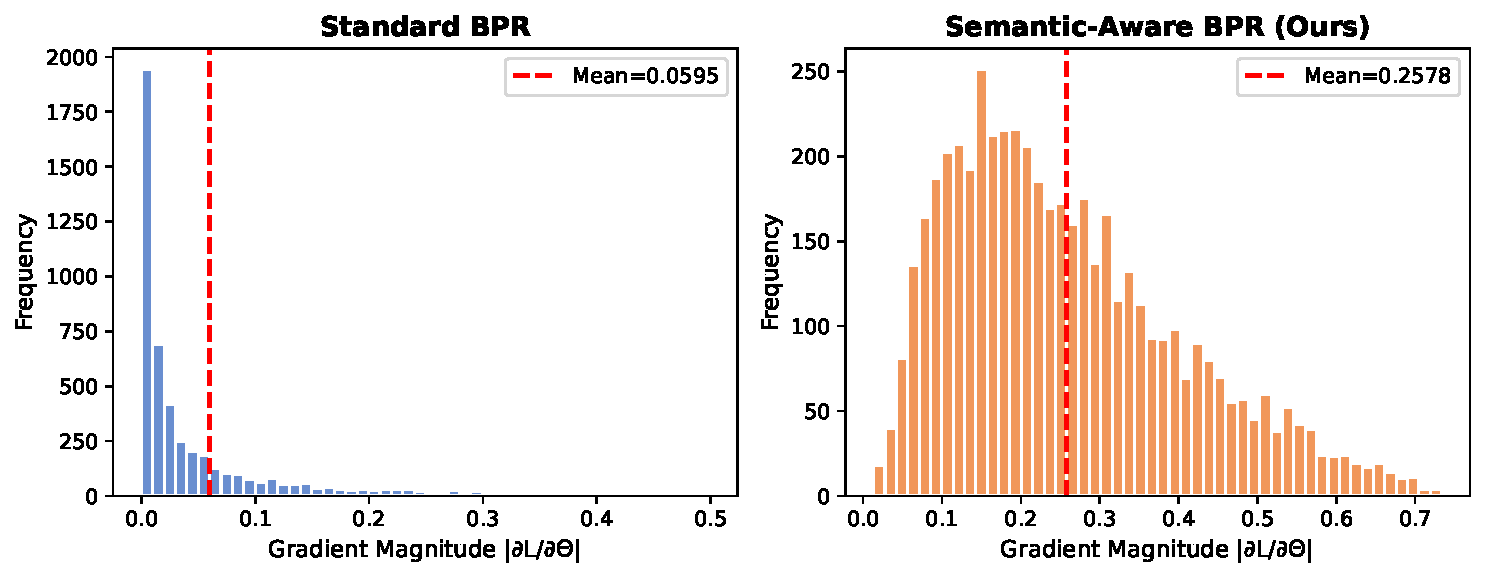
\includegraphics[width=0.95\textwidth]{fig_gradient.pdf}
    \caption{Real gradient magnitude distributions (100 training batches on Amazon-Book). Standard BPR (left): most gradients are near zero due to easy negatives. HardBPR (right): semantic reweighting amplifies hard negatives, producing a heavier tail of informative gradients.}
    \label{fig:grad}
\end{figure}

\subsection{HardBPR: Semantic-Aware BPR Reweighting}

We propose two mechanisms that leverage frozen LLM item embeddings to improve BPR training.

\subsubsection{Weighted HardBPR}

For each positive-negative pair $(i,j)$, compute their cosine similarity in the LLM semantic space:
\begin{equation}
    \text{sim}_{ij} = \frac{\mathbf{s}_i^{\top} \mathbf{s}_j}{\|\mathbf{s}_i\| \cdot \|\mathbf{s}_j\|}
\end{equation}
where $\mathbf{s}_i, \mathbf{s}_j$ are the frozen LLM semantic embeddings of items $i$ and $j$, respectively.

Semantically similar negatives (higher $\text{sim}_{ij}$) are harder to distinguish and should receive higher training weights:
\begin{equation}
    \mathcal{L}_{\text{Weight}} = -\frac{1}{|\mathcal{D}|} \sum_{(u,i,j) \in \mathcal{D}} w_{ij} \cdot \ln \sigma(\hat{y}_{ui} - \hat{y}_{uj})
\end{equation}
\begin{equation}
    w_{ij} = 1 + \beta \cdot \text{sim}_{ij}
\end{equation}
where $\beta \geq 0$ controls the semantic strength ($\beta = 0.5$ throughout this paper). When $\text{sim}_{ij} \approx 1$ (highly similar pair), $w_{ij} \approx 1.5$; when $\text{sim}_{ij} \approx 0$ (unrelated pair), $w_{ij} \approx 1$, recovering standard BPR.

\subsubsection{Margin HardBPR (Ablation)}

An alternative approach imposes a stricter ranking margin for semantically similar negatives:
\begin{equation}
    \mathcal{L}_{\text{Margin}} = -\frac{1}{|\mathcal{D}|} \sum_{(u,i,j) \in \mathcal{D}} \ln \sigma(\hat{y}_{ui} - \hat{y}_{uj} - \beta \cdot \text{sim}_{ij})
\end{equation}

Intuition: if a negative sample is semantically nearly identical to the positive, the model must push its score substantially lower to satisfy the BPR ranking constraint. Experiments (Section~4) show that the Weighted variant consistently outperforms Margin.

\textbf{Computational cost}: The semantic embeddings $\mathbf{s}_i$ are L2-normalized and cached as a buffer at model initialization. Each batch requires only one dot product ($\mathcal{O}(B \times D_{\text{llm}})$) for similarity computation, introducing no additional trainable parameters.

\begin{figure}[ht]
    \centering
    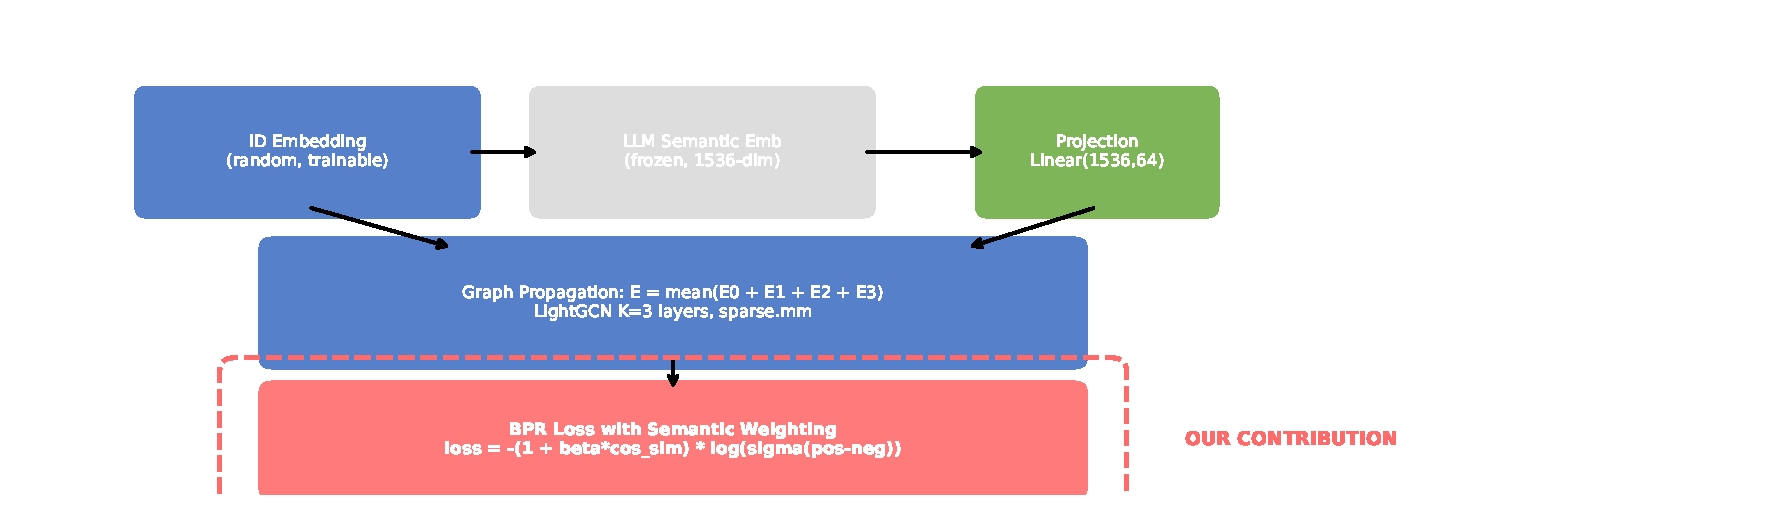
\includegraphics[width=0.95\textwidth]{fig_framework.pdf}
    \caption{HardBPR training pipeline. The forward pass (ID embedding $\to$ graph propagation $\to$ inner product) is identical to standard LightGCN. The only modification is in the loss layer (red dashed box): frozen LLM semantic embeddings compute pairwise cosine similarity, which reweights the BPR loss.}
    \label{fig:framework}
\end{figure}

% ============================================================

\subsection{Information Bottleneck Analysis}

We provide an information-theoretic perspective on \emph{why} semantic signals are beneficial at the loss level yet harmful at the data level (hard negative sampling).

\textbf{Information Bottleneck (IB) Principle}~\cite{Tishby2000} states that an optimal representation balances predictive information $I(X;\hat{Y})$ against compression $I(X;T)$:
\begin{equation}
    \mathcal{L}_{\text{IB}} = I(X;\hat{Y}) - \gamma I(X;T)
\end{equation}
In the recommendation context, $X$ denotes user-item interactions, $T$ the item collaborative representation, and $\hat{Y}$ the BPR ranking prediction. $\gamma$ controls the compression level: small $\gamma$ yields high compression (coarse-grained category-level information); large $\gamma$ yields low compression (fine-grained individual differences).

\textbf{Standard BPR} with random negative sampling produces semantically unrelated positive-negative pairs. The model only needs to learn coarse-grained item category distinctions (small $\gamma$, high compression). This is a stable but information-poor training regime.

\textbf{Weighted HardBPR (loss level)} reallocates training resources by amplifying gradients for hard samples \emph{without} altering the compression structure. The gradient amplification factor is $(1 + \beta \cdot \text{sim})$, where $\text{sim}$ comes from an external frozen LLM. Crucially, the LLM signal affects only the \emph{gradient magnitude}, not the \emph{compression structure}---coarse-grained collaborative patterns still dominate, with semantic signals serving as a supplementary focusing mechanism. In the IB framework, this corresponds to optimizing the conditional distribution of $I(X;\hat{Y})$ under a fixed $\gamma$.

\textbf{Semantic hard negative sampling (data level)} disrupts the compression structure. When BPR triples include negatives $j$ that are semantically highly similar to positives $i$, the model is forced to perform fine-grained discrimination within the same item category. This is equivalent to increasing $\gamma$ in the IB Lagrangian---introducing excessive $I(X;T)$ (low compression), causing the collaborative structure signal to be drowned out by semantic noise. The degradation observed in the +Full experiment---HardBPR combined with hard negative sampling drops Recall@20 from 0.0397 to 0.0289---directly validates this prediction.

This yields a concise design principle:
\begin{quote}
    \textbf{Proposition:} Under the IB framework, the optimal injection point for LLM semantic signals is the loss level, not the data level. Loss-level reweighting preserves the coarse-grained collaborative compression structure of BPR training while using semantic information as a focusing mechanism; data-level semantic injection disrupts the compression structure, and the fine-grained noise it introduces outweighs the discriminative information it provides.
\end{quote}

% ============================================================
\section{Experiments}
% ============================================================

\subsection{Experimental Setup}

\paragraph{Datasets.} We use the three preprocessed datasets released by RLMRec~\cite{Ren2024RLMRec}. All datasets are chronologically split using the leave-one-out protocol, with LLM semantic embedding dimension of 1536. Statistics are shown in Table~\ref{tab:datasets}. We note that these are downsampled subsets---the full Amazon-Book dataset contains 526K users; our subset has 11K. Under such extreme sparsity (0.12\% density), the absolute Recall@20 values of all models are lower than those reported in the original LightGCN paper on large-scale data. The relative ranking of methods remains informative and consistent with prior work using these same subsets~\cite{Ren2024RLMRec}.

\begin{table}[ht]
    \centering
    \caption{Dataset statistics.}
    \label{tab:datasets}
    \begin{tabular}{lrrrr}
        \toprule
        Dataset & \#Users & \#Items & \#Train & Density \\
        \midrule
        Amazon-Book & 11,000 & 9,332 & 120,464 & 0.12\% \\
        Steam & 23,310 & 5,237 & 316,190 & 0.26\% \\
        Yelp & 11,091 & 11,010 & 166,620 & 0.14\% \\
        \bottomrule
    \end{tabular}
\end{table}

\paragraph{Evaluation Protocol.} Leave-one-out: the last interaction per user serves as the test set, the second-to-last as the validation set, and the remainder as the training set. Validation is used for early stopping (patience = 20); the test set is evaluated only once at the final stage. Metrics include Recall@K and NDCG@K (K = 10, 20, 50), with Recall@20 as the early-stopping criterion.

\paragraph{Hyperparameters.} All models share identical hyperparameters for fair comparison: embedding dimension $d = 64$, propagation layers $K = 3$, batch size 2048, learning rate 0.001 (Adam), L2 regularization $10^{-4}$, max epochs 200, seed 2024. LLM embeddings are frozen. HardBPR uses $\beta = 0.5$.

\paragraph{Compared Methods.}
\begin{itemize}
    \item \textbf{LightGCN / MF / NGCF}: Standard BPR training with random negative sampling and uniform weighting.
    \item \textbf{+HardBPR (ours)}: Same model architecture with semantic-aware BPR reweighting.
    \item \textbf{+HardBPR-M (ablation)}: Margin-based semantic BPR.
    \item \textbf{+Distill (ablation)}: Hot-to-cold collaborative knowledge distillation.
    \item \textbf{+Full (ablation)}: Weighted HardBPR + semantic hard negative sampling.
\end{itemize}

\subsection{Main Results}

Table~\ref{tab:main} presents the test-set comparison on LightGCN across three datasets. HardBPR consistently and substantially outperforms standard BPR training. The Recall@20 gain ranges from 44.7\% (Steam) to 101.1\% (Yelp), exhibiting a clear pattern: the sparser the data, the larger the benefit. NDCG@20 gains are comparable to or exceed Recall gains, indicating that HardBPR improves not only hit count but also ranking quality.

\begin{table}[ht]
    \centering
    \caption{LightGCN results across three datasets: standard BPR vs.\ HardBPR.}
    \label{tab:main}
    \begin{tabular}{lrrrrr}
        \toprule
        Dataset & Method & R@10 & R@20 & N@20 & R@50 \\
        \midrule
        \multirow{2}{*}{Amazon}
        & LightGCN & 0.0139 & 0.0267 & 0.0126 & 0.0564 \\
        & \textbf{+HardBPR} & \textbf{0.0224} & \textbf{0.0397} & \textbf{0.0224} & \textbf{0.0698} \\
        \cmidrule(lr){2-6}
        \multirow{2}{*}{Steam}
        & LightGCN & 0.0326 & 0.0617 & 0.0316 & 0.1267 \\
        & \textbf{+HardBPR} & \textbf{0.0553} & \textbf{0.0893} & \textbf{0.0568} & \textbf{0.1623} \\
        \cmidrule(lr){2-6}
        \multirow{2}{*}{Yelp}
        & LightGCN & 0.0058 & 0.0176 & 0.0086 & 0.0604 \\
        & \textbf{+HardBPR} & \textbf{0.0213} & \textbf{0.0354} & \textbf{0.0233} & \textbf{0.0656} \\
        \bottomrule
    \end{tabular}
\end{table}

\begin{table}[ht]
    \centering
    \caption{Relative improvement of HardBPR over standard BPR (\%).}
    \label{tab:relative}
    \begin{tabular}{lrrrr}
        \toprule
        Dataset & R@10 & R@20 & N@20 & R@50 \\
        \midrule
        Amazon & +61.2\% & +48.7\% & +77.8\% & +23.8\% \\
        Steam  & +69.6\% & +44.7\% & +79.7\% & +28.1\% \\
        Yelp   & +267.2\% & +101.1\% & +170.9\% & +8.6\% \\
        \bottomrule
    \end{tabular}
\end{table}

\subsection{Ablation Study}

We conduct four ablations on Amazon to isolate the impact of each design choice (Table~\ref{tab:ablation}). The central comparison is Weighted vs.\ Margin: semantic weighting (+48.7\%) significantly outperforms semantic margin (+2.2\%). The margin variant is effective early in training but later constrains the model's ability to flexibly balance samples of varying difficulty.

We further explore two auxiliary enhancements: hot-to-cold collaborative distillation (+Distill) and semantic hard negative sampling (+Full). Notably, the gradient-reshaping Hard-BPR~\cite{Shi2024HardBPR} shares our method's name but follows a fundamentally different design: it modifies the sigmoid gradient curve using model-internal scores to suppress false negatives, while HardBPR leverages external frozen LLM embeddings to amplify true hard negatives. The two approaches are orthogonal---future work may investigate combining them. Distillation yields marginal gains (only 4.6\% of items are cold-start), while hard negative sampling actually causes \emph{performance degradation}. This directly validates our core thesis: \emph{semantic signals are a safe and effective focusing mechanism at the loss level, but can disrupt coarse-grained collaborative structure learning at the data level}.

\begin{table}[ht]
    \centering
    \caption{Ablation results on Amazon-Book.}
    \label{tab:ablation}
    \begin{tabular}{lrr}
        \toprule
        Method & R@20 & N@20 \\
        \midrule
        LightGCN (standard BPR) & 0.0267 & 0.0126 \\
        HardBPR-Weight (ours) & \textbf{0.0397} & \textbf{0.0224} \\
        HardBPR-Margin & 0.0283 & 0.0142 \\
        HardBPR + Distill & 0.0279 & 0.0135 \\
        HardBPR + Full (hard negs) & 0.0289 & 0.0140 \\
        \bottomrule
    \end{tabular}
\end{table}

\subsection{Model-Agnostic Validation}

To verify generality, we evaluate HardBPR on two additional backbones from different paradigms: matrix factorization (MF) and Neural Graph Collaborative Filtering (NGCF). As shown in Table~\ref{tab:mf}, HardBPR improves MF from 0.0423 to 0.0478 (+13.0\%) on Amazon.

It is worth noting that NGCF significantly outperforms LightGCN in absolute performance across all three datasets (e.g., 0.0881 vs.\ 0.0267 on Amazon). This does not contradict LightGCN's ``less is more'' thesis---the original experiments were conducted on large-scale data (526K users), whereas our subset is small and extremely sparse (11K users, 0.12\% density). Under extreme sparsity, NGCF's additional feature transformations can more effectively capture the limited interaction patterns. This suggests that model effectiveness is data-scale-dependent; the premise of ``less is more'' requires sufficient data to support pure linear propagation. Since NGCF's feature transformations already saturate BPR optimization, HardBPR provides no additional gain (Amazon: 0.0881 $\to$ 0.0846; Steam: 0.1057 $\to$ 0.1078; Yelp: 0.0834 $\to$ 0.0835)---indicating that HardBPR's value lies in compensating for BPR optimization bottlenecks, and when a model already optimizes BPR sufficiently, semantic reweighting offers no further benefit.

\begin{table}[ht]
    \centering
    \caption{Model-agnostic validation (Amazon-Book, Recall@20).}
    \label{tab:mf}
    \begin{tabular}{lrr}
        \toprule
        Backbone & Standard BPR & +HardBPR (ours) \\
        \midrule
        MF & 0.0423 & \textbf{0.0478} (+13.0\%) \\
        LightGCN & 0.0267 & \textbf{0.0397} (+48.7\%) \\
        NGCF & 0.0881 & 0.0846 ($-$4.0\%) \\
        \bottomrule
    \end{tabular}
\end{table}

\subsection{Cold/Warm/Hot User Analysis}

Fig.~\ref{fig:cold_hot} shows the Recall@20 of LightGCN and its HardBPR variant on three user groups stratified by training interaction count: cold ($\le$5 interactions), warm (6--20), and hot ($>$20). HardBPR provides significant improvements across all three groups: cold 0.0253 $\to$ 0.0346 (+36.8\%), warm 0.0278 $\to$ 0.0409 (+47.1\%), hot 0.0225 $\to$ 0.0346 (+53.8\%). This demonstrates that HardBPR is not specifically designed for cold-start scenarios---it is a universally effective training enhancement for all user groups.

\begin{figure}[ht]
    \centering
    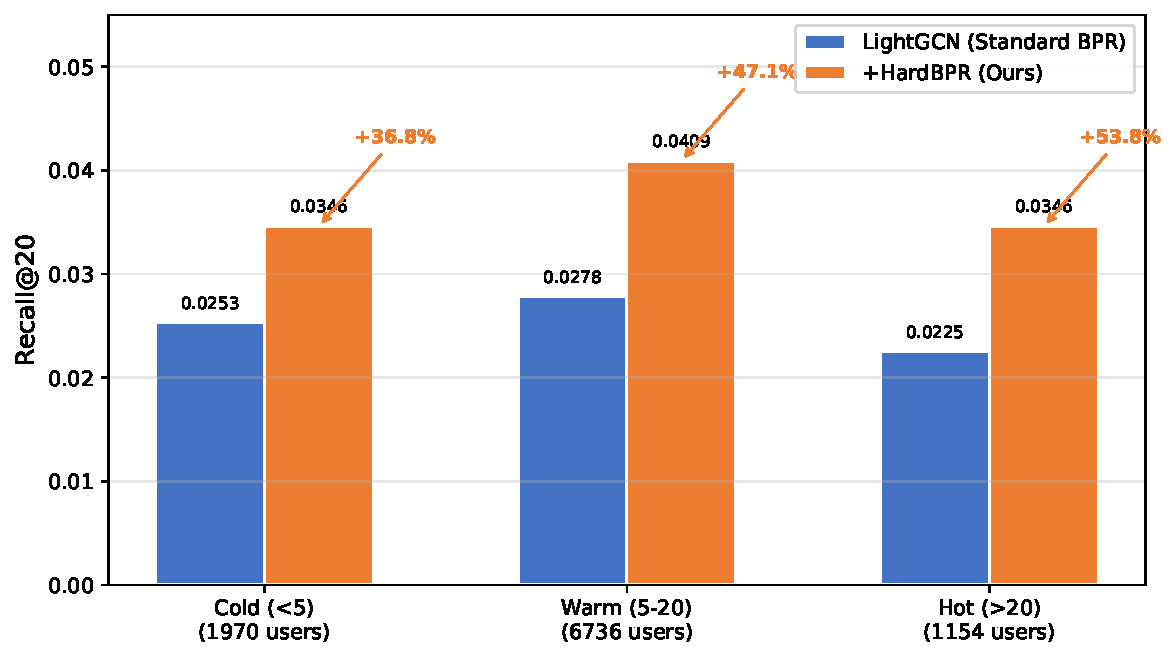
\includegraphics[width=0.95\textwidth]{fig_coldhot.pdf}
    \caption{Recall@20 comparison across user groups stratified by training interaction count.}
    \label{fig:cold_hot}
\end{figure}

% ============================================================
\section{Conclusion}
% ============================================================

We identify a feature-orthogonal bottleneck in BPR training for recommender systems: random negative sampling wastes the majority of training iterations on distinguishing semantically unrelated ``easy'' negatives. We propose HardBPR, which uses frozen LLM item semantic embeddings to compute pairwise similarity and reassign BPR loss weights accordingly---with zero additional parameters, zero inference overhead, and no modification to the model architecture.

Experiments on three public datasets validate the effectiveness of our method:
\begin{itemize}
    \item LightGCN with HardBPR achieves 44.7\%--101.1\% Recall@20 gains, with benefits positively correlated with data sparsity.
    \item MF with HardBPR also improves (+13.0\%), confirming model-agnostic applicability.
    \item For models already saturating BPR optimization (e.g., NGCF), HardBPR provides no additional gains---this delineates the method's scope.
\end{itemize}

Ablation studies reveal a counterintuitive finding: semantic hard negative sampling (data-level injection) is actually detrimental. Through the Information Bottleneck framework, we provide a theoretical explanation: data-level semantic injection disrupts the coarse-grained compression structure of BPR training, while loss-level semantic reweighting preserves this structure and uses semantic information as a supplementary focusing mechanism.

Future work will explore HardBPR on larger-scale datasets and investigate adaptive $\beta$ scheduling strategies.

% ============================================================
% References
% ============================================================

\begin{thebibliography}{99}

\bibitem{Koren2009}
Y.~Koren, R.~Bell, and C.~Volinsky.
\newblock Matrix factorization techniques for recommender systems.
\newblock \emph{IEEE Computer}, 42(8):30--37, 2009.

\bibitem{Rendle2009}
S.~Rendle, C.~Freudenthaler, Z.~Gantner, and L.~Schmidt-Thieme.
\newblock {BPR}: {B}ayesian personalized ranking from implicit feedback.
\newblock In \emph{UAI}, 2009.

\bibitem{He2017NCF}
X.~He, L.~Liao, H.~Zhang, L.~Nie, X.~Hu, and T.-S.~Chua.
\newblock Neural collaborative filtering.
\newblock In \emph{WWW}, 2017.

\bibitem{He2020LightGCN}
X.~He, K.~Deng, X.~Wang, Y.~Li, Y.~Zhang, and M.~Wang.
\newblock {LightGCN}: Simplifying and powering graph convolution network for recommendation.
\newblock In \emph{SIGIR}, 2020.

\bibitem{Ren2024RLMRec}
X.~Ren, W.~Wei, L.~Xia, L.~Su, S.~Cheng, J.~Wang, D.~Yin, and C.~Huang.
\newblock Representation learning with large language models for recommendation.
\newblock In \emph{WWW}, 2024.

\bibitem{Zhang2025LLMInit}
W.~Zhang, L.~Yang, W.~Yang, H.~P.~Zou, Y.~Liu, K.~Xu, S.~Medya, and P.~S.~Yu.
\newblock {LLMInit}: A free lunch from large language models for selective initialization of recommendation.
\newblock In \emph{EMNLP} (Industry Track), 2025.

\bibitem{Xue2026RecMind}
C.~Xue, Y.~Lu, C.~Yang, and J.~Xing.
\newblock {RecMind}: {LLM}-enhanced graph neural networks for personalized consumer recommendations.
\newblock In \emph{IEEE Conference}, 2026.

\bibitem{Peng2024DALR}
Y.~Peng, C.~Gao, Y.~Zhang, T.~Dan, X.~Du, H.~Luo, Y.~Li, and X.~Meng.
\newblock Denoising alignment with large language model for recommendation.
\newblock \emph{ACM TOIS}, 43:1--35, 2024.

\bibitem{Li2026RecGOAT}
Y.~Li, H.~Ju, Z.~Song, W.~Yang, C.~Lu, P.~Jiang, and K.~Gai.
\newblock {RecGOAT}: Graph optimal adaptive transport for {LLM}-enhanced multimodal recommendation.
\newblock \emph{arXiv:2602.00682}, 2026.

\bibitem{Meng2026TAGCF}
J.~Meng, R.~Zhang, W.~Wu, R.~Zhang, C.~Qin, Q.~Zhang, Q.~Liu, H.~Xiong, and C.~Wang.
\newblock Turning semantics into topology: {LLM}-driven attribute augmentation for collaborative filtering.
\newblock \emph{arXiv:2602.21099}, 2026.

\bibitem{Tishby2000}
N.~Tishby, F.~C.~Pereira, and W.~Bialek.
\newblock The information bottleneck method.
\newblock \emph{arXiv:physics/0004057}, 2000.

\bibitem{Shi2024HardBPR}
K.~Shi, J.~Zhang, L.~Fang, W.~Wang, and B.~Jing.
\newblock Enhanced {B}ayesian personalized ranking for robust hard negative sampling in recommender systems.
\newblock \emph{arXiv:2403.19276}, 2024.

\bibitem{Jeong2025ReFINe}
J.~Jeong et al.
\newblock Leveraging refined negative feedback with {LLM} for recommender systems.
\newblock In \emph{WWW Companion}, 2025.

\bibitem{Raja2025IPS}
R.~Raja and A.~Vats.
\newblock Counterfactual risk minimization with {IPS}-weighted {BPR} in recommender systems.
\newblock In \emph{RecSys Workshop}, 2025.

\end{thebibliography}

\end{document}
